% 
% ======================================================================
\RequirePackage{docswitch}
% \flag is set by the user, through the makefile:
%    make note
%    make apj
% etc.
\setjournal{\flag}

\documentclass[\docopts]{\docclass}

% You could also define the document class directly
%\documentclass[]{emulateapj}

% Custom commands from LSST DESC, see texmf/styles/lsstdesc_macros.sty
\usepackage{lsstdesc_macros}

\usepackage{graphicx}
\graphicspath{{./}{./figures/}}
\bibliographystyle{apj}
\usepackage{subfigure}

% Add your own macros here:



% 
% ======================================================================

\begin{document}

\title{ On the cadence of the LSST SN survey(s) }

\maketitlepre

\begin{abstract}

Design notes, metrics and forecasts for the deep and wide LSST SN surveys.

\end{abstract}

% Keywords are ignored in the LSST DESC Note style:
\dockeys{latex: templates, papers: awesome}

\maketitlepost

% ----------------------------------------------------------------------
% 

\section{Introduction}
\label{sec:intro}

LSST has the capability to discover $O(10^5)$ SNe~Ia in the redshift
range $0.03 < z < 0.4$ (wide survey) and $0.3 < z < 1.1$ (DDF
survey). The question of how many of these events will have light
curves of sufficient quality to be included in a Hubble diagram
remains open.  It is essentially a function of the cadence and depth
that will be delivered by the Wide and DDF surveys.

In this note, we examine the cadence envisioned for the 10 years of
LSST operations.  We base ourselves



% This is a paper and note template for the LSST DESC
% \citep{Overview,ScienceBook,WhitePaper}.  You can delete all this
% tutorial text whenever you like.

% You can easily switch between various \LaTeX\xspace styles for
% internal notes and peer reviewed journals.  Documents can be
% compiled using the provided \code{Makefile}.  The command
% \code{make} with no arguments compiles \code{main.tex} using the
% \code{lsstdescnote.cls} style.  If you want to upgrade your Note
% into a journal article, just choose a journal name, between
% \code{make apj} (ApJ preprint format), \code{make apjl} (which uses
% the \code{emulateapj} style), \code{make prd}, \code{make prl}, and
% \code{make mnras}.


% ----------------------------------------------------------------------

\section{Design notes}
\label{sec:design_notes}

\paragraph{Redshift-limited survey} A key design quantity is the
redshift limit ($z_{lim}$) of the survey. Here, we do not refer to a
detectability limit, but to the redshift value beyond which we start
losing a fraction of the sample, because the follow-up is not good
enough (1) to measure a distance and (2) to perform a photometric
identification.  Beyond this redshift limit, one has to estimate the
fraction of events lost. This procedure yields uncertainties, that are
quite intricated with (1) the control of the demographic evolution of
SNe~Ia (2) the standardization procedures (see impact on $\beta$).  As
a consequence, the supernovae beyond $z_{lim}$ are of limited
usefulness.  Rather, we need to define, for each of our two surveys
(DDF and wide) a nominal $z_{lim}$, and aim at building a sample that
is complete up to $z_{lim}$. 

By ``complete'', we mean that, each SN~Ia occurring:
\begin{itemize}
\item in a well defined observer-frame time interval (that corresponds
  to a season) $[T_{start}; T_{end}]$;
\item in the redshift range $0.05 < z < z_{lim}$;
\item in a region of the SN~Ia parameter space that is large enough to
  encompass a potential evolution with redshift of the SN~Ia
  demographic properties;
\end{itemize}
has a follow-up which is ``good enough'' to (1) identify it
photometrically as a SN~Ia and (2) derive a standardized distance from
its lightcurve.

\paragraph{Fiducial SN~Ia parameter space region} Up to a good
approximation, SNe~Ia form a 2-dimensional family, that may be indexed
for example with color and lightcurve-width (for example, the
SALT2-color and the SALT2-$X1$-parameter).  On figure
\ref{fig:jla_X1_C}, we show the distribution of the JLA supernovae, in
the $(X1,C)$ parameter space. We note sizeable differences between the
nearby and distant SNe, in particular in X1.  However, the full JLA
sample is well contained in the region $X1 = [-3,3], Color= = [-0.3,
0.3]$. 

\begin{figure}[t]
\begin{center}
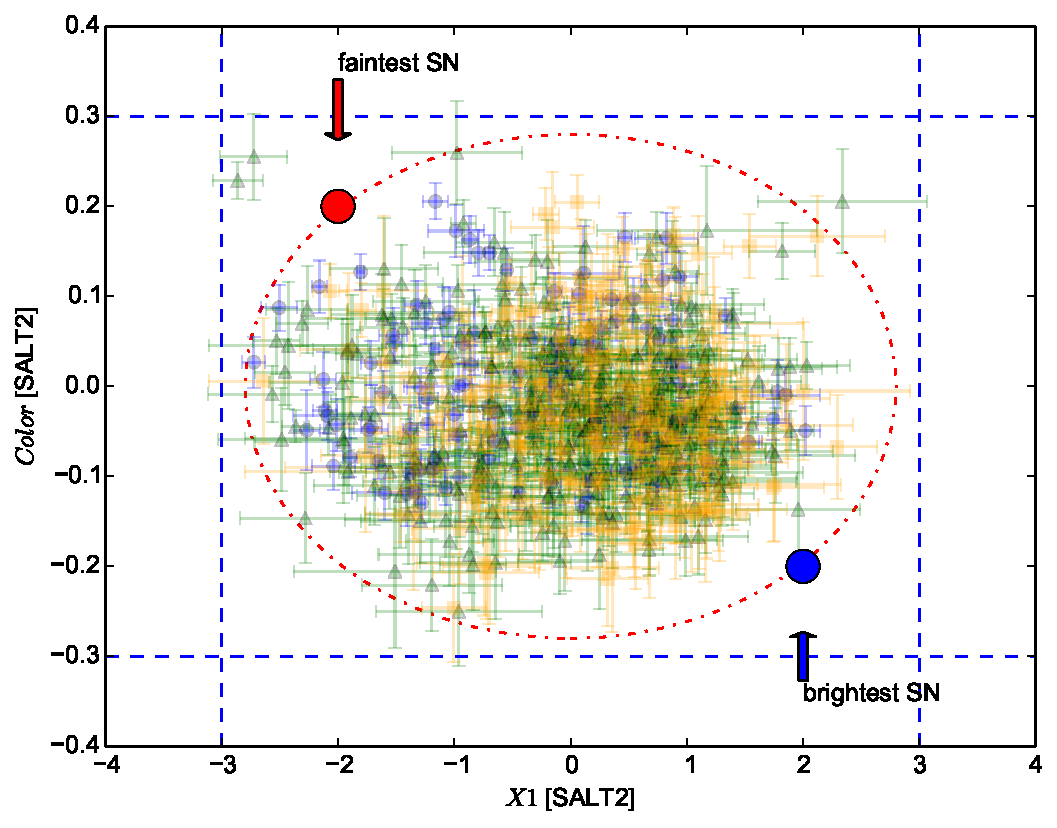
\includegraphics[width=0.75\linewidth]{sn_parameter_space.pdf}
\caption{JLA supernovae the $(X1,Color)$ parameter space -- (blue:
  nearby, green: SDSS, orange: SNLS).  }
\label{fig:jla_X1_C}
\end{center}
\end{figure}

On the same figure, we have marked in red the faintest SN in that
parameter space ($X1=-3, Color=0.3$). To be complete up to $z_{lim}$,
the survey has to deliver a cadence that allows to derive a luminosity
distance and a photometric identification for that event at a redshift
$z_{lim}$.

\paragraph{Lightcurve quality requirements} Our lightcurve quality
requirements are as follows:

\begin{equation}
  \mu = m^\star_B + \alpha X_1 - \beta C
\end{equation}

\begin{itemize}
\item we need measurements in at least two bands, in order to
  constrain the restframe color of the SN. Given the high intrinsic
  dispersions of SNe~Ia in the restframe UV, these bands must sample
  to the restframe region $3800 \angstrom < \lambda < 7000 \angstrom$.

\item we require the light curve shape to be well sampled in the
  (restframe) phase interval $[-10;+30]$ days, with at least four
  visits before peak (each of those visits in any of the eligible
  band), and ten visits after peak.
  
\item finally, we require that the photon noise contribution to the
  distance measurement is subdominant w.r.t. the intrinsic dispersion
  of the SNe (after standardization).  There are several ways to
  quantify this.  The dominant contribution is carried by the color
  (since $\beta \sim 3$). This means that requiring $\sigma C < 0.03$
  ensures that $\sigma \mu < 0.1$, below the intrinsic dipersion in
  the Hubble diagram, after standardization.

  Another way to look at this consists in placing requirements on the
  uncertainty of the amplitude of the lightcurve shape. 
\end{itemize}


Our goal is to make sure that the light curves of our faintest
$(X1=-3, C=0.3)$ SNe~Ia around $z = z_{lim}$ pass these requirements.







% There are a number of useful \LaTeX\xspace commands predefined in
% \code{macros.tex}.  Notice that the section labels are prefixed with
% \code{sec:} to allow the use of the \verb=\secref= command to
% reference a section (\ie, \secref{intro}).  Figures can be referenced
% with the \verb=\figref= command, which assumes that the figure label
% is prefixed with \code{fig:}.  In \figref{example} we show an example
% figure.  You'll notice that the actual figure file is found in the
% \code{figures} directory.  However, because we have specified this
% directory in our \verb=\graphicspath= we do not need to explicitly
% specify the path to the image.

% The \code{macros.tex} package also contains some conventional
% scientific units like \angstrom, \GeV, \Msun, etc. and some editorial
% tools for highlighting \FIXME{issues}, \CHECK{text to be checked},
% \COMMENT{comments}, and \NEW{new additions}.


% ----------------------------------------------------------------------

\section{A simple metric to evaluate a cadence}
\label{sec:methods}



% Similar to the figure before, here we have included a table of data
% from \code{tables/table.tex}.  Notice that again we are able to
% reference \tabref{example} with the \verb=\tabref= command using the
% \code{tab:} prefix.  Also notice that we haven't needed to specify the
% full path to the table because in the \code{Makefile} we include
% \code{./tables} directory in the \code{\$TEXINPUTS} environment
% variable.

% \begin{table}
  \begin{center}
  \caption{Example table. \label{tab:example}}
  %\begin{ruledtabular}
  \begin{tabular}{lccc}
\hline\hline
Column 1 & Column 2 & Column 3 &  Column 4 \\[3pt]  
     &    $\deg$     & $\kpc$   &  $\deg$ \\[4pt]
\hline
Obj1 & (0,0) & 10 & 0.1 \\
... & ... & ... & ... \\
ObjN & (0,0) & 10 & 0.1
\\\hline\hline
\end{tabular}
\end{center}
%\end{ruledtabular}
\end{table}

%\begin{\tabletype}{l ccccccc }
%\tablewidth{0pt}
%\tabletypesize{\tiny}
%\tablecaption{ An example table. \label{tab:example}}
%\tablehead{
%(1) & (2) & (3) & (4) & (5) & (6) & (7) & (8)\\
%Name & GLON,GLAT & Distance & $r_{1/2}$ & $\log_{10}(J_{\rm meas})$ & $\log_{10}(J_{\rm pred})$ & Sample & Refrence \\
% & (deg) & (kpc) & (pc) & $\log_{10}(\GeV^2 \cm^{-5})$ & $\log_{10}(\GeV^2 \cm^{-5})$ & & 
%}
%\startdata
%Bootes I                     & 358.08,69.62   & 66  & 189  & $18.8 \pm 0.2$ & 18.5           & I,S,C & ... \\
%\\
%...\\
%\\
%Willman 1                    & 158.58,56.78   & 38  & 19   & $19.1 \pm 0.3$ & 18.9           & I,S & ... \\
%\enddata
%{\footnotesize \tablecomments{ (1) The first column. (2) The second column ...}}
%\end{\tabletype}


% Equations appear as follows, and can be referred to as, for example, \eqnref{example} -- just as for tables, we use the \verb=\eqnref= command using the \code{eqn:} prefix.
% \begin{equation}
%   \label{eqn:example}
%   \langle f(k) \rangle = \frac{ \sum_{t=0}^{N}f(t,k) }{N}
% \end{equation}


% ----------------------------------------------------------------------
\section{The DEEP LSST SN survey}

\subsection{The DDF cadence from \code{Minion\_1016}}
\label{sec:results}

% \figref{example} shows an example figure, referred to with the \verb=\figref= command and the \code{fig:} prefix.

% \begin{figure}
% 
\includegraphics[width=0.9\columnwidth]{example.png}
% \caption{An example figure: the LSST DESC logo, copied from \code{texmf/logos/desc-logo.png} into \code{figures/example.png}. \label{fig:example}}
% \end{figure}


% ----------------------------------------------------------------------
\section{The Wide LSST SN survey}
\subsection{The cadence from \code{Minion\_1016}}
\label{sec:results}

% \figref{example} shows an example figure, referred to with the \verb=\figref= command and the \code{fig:} prefix.

% \begin{figure}
% 
\includegraphics[width=0.9\columnwidth]{example.png}
% \caption{An example figure: the LSST DESC logo, copied from \code{texmf/logos/desc-logo.png} into \code{figures/example.png}. \label{fig:example}}
% \end{figure}

\subsection{The rolling cadence from \code{Minion\_1016}}
\label{sec:results}

% ----------------------------------------------------------------------

\section{The Rolling Cadence }
\label{sec:results}

% \figref{example} shows an example figure, referred to with the \verb=\figref= command and the \code{fig:} prefix.

% \begin{figure}
% 
\includegraphics[width=0.9\columnwidth]{example.png}
% \caption{An example figure: the LSST DESC logo, copied from \code{texmf/logos/desc-logo.png} into \code{figures/example.png}. \label{fig:example}}
% \end{figure}




% ----------------------------------------------------------------------

\section{Discussion}
\label{sec:discussion}

If you are planning on committing your paper to GitHub, it's a good idea to write your tex as one sentence per line.
This allows for an easier \code{diff} of changes.
It also makes sense to think of latex as \emph{code}, and sentences as logical statements, occupying one line each.
Each line must ``compile'' in the mind of the reader.


% ----------------------------------------------------------------------

\section{Conclusions}
\label{sec:conclusions}

Here's a summary of what we just reported.

We can draw the following well-organized and neatly-formatted conclusions:
\begin{itemize}
  \item This is important.
  \item We can measure some number with some precision.
  \item This has some implications.
\end{itemize}

Here are some parting thoughts.


% ----------------------------------------------------------------------

\subsection*{Acknowledgments}

Here is where you should add your specific acknowledgments, remembering that some standard thanks will be added via the \code{acknowledgments.tex} and \code{contributions.tex} files.

% 
This is the text imported from \code{acknowledgments.tex}, and will be replaced by some standard LSST DESC boilerplate at some point.
% 


\input{contributions}

%{\it Facilities:} \facility{LSST}

% Include both collaboration papers and external citations:
\bibliography{lsstdesc,main}


\appendix

\section{LSST instrument models}

To prepare this study, we have used two instrument models.  One is
based on the numbers reported in \cite[][LSE-40 hereafter]{LSE-40}.
We report the main ingredients of this model in table \ref{tab:lse40}. 

The other model is described in \cite[][hereafter
SMTN-002)]{SMTN-002}, which constitutes a preliminary update of
LSE-40.  The current version OpSim relies on SMTN-002. An we therefore
adopt this model as our reference. Key quantities of SMTN-002 are
listed in table \ref{tab:smtn002}.

We note that both models differ very significantly. In particular (1)
the throughput of SMTN-002 is almost 50\% lower.


\begin{table}
\begin{center}
\caption{LSE-40 model}
\label{tab:lse40}
\begin{tabular}{l|cccccc}
\hline 
\hline 
\multicolumn{7}{c}{{\bf General}} \\
\hline
Pixel size & \multicolumn{6}{r}{0.2 arcsec} \\
RO noise   & \multicolumn{6}{r}{9 $e^-$}    \\
\hline
\multicolumn{7}{c}{{\bf Zero Points @ X=1 [AB, fluxes in e$^-$/s]}} \\
\hline
           &  $u$ & $g$ & $r$ & $i$ & $z$ & $y$ \\
LSE-40     & 27.09 & 28.58 & 28.50 & 28.34 & 27.95 & 27.18 \\
snsim      & 27.05 & 28.59 & 28.53 & 28.38 & 27.99 & 27.22 \\
\hline
\multicolumn{7}{c}{{\bf median seeing [arcsec]}} \\
\hline
LSE-40 / snsim  &  0.77 &  0.73 &  0.70 &  0.67 &  0.65 &  0.63 \\
\hline
\multicolumn{7}{c}{{\bf Dark sky [AB mag / arcsec$^2$]}}   \\
\hline
LSE-40     & 22.92 & 22.27 & 21.20 & 20.47 & 19.59 & 18.63 \\
snsim      & 22.95 & 22.26 & 21.20 & 20.47 & 19.60 & 18.61 \\
\hline
\multicolumn{7}{c}{{\bf NEA [pixel$^2$]}}   \\
\hline
snsim (Moffat, $\beta=4.5$)     & 41.5  & 37.4  & 34.5  & 31.7 & 29.9  & 28.6  \\
\hline
\multicolumn{7}{c}{{\bf Limiting mag ($5 \sigma$), 30-s visit}}   \\
\hline
LSE-40                        & 24.22  &  25.15 &  24.74  &  24.38  &  23.80  &  22.93  \\
snsim (Moffat, $\beta=7$)     & 24.27  &  25.18 &  24.73  &  24.36  &  23.77  &  22.92  \\
\hline
\end{tabular}
\end{center}
\end{table}


\begin{table}
\begin{center}
\caption{SMTN-002 model}
\label{tab:smtn002}
\begin{tabular}{l|cccccc}
\hline 
\hline 
\multicolumn{7}{c}{{\bf General}} \\
\hline
Pixel size & \multicolumn{6}{r}{0.2 arcsec} \\
RO noise   & \multicolumn{6}{r}{9 $e^-$}    \\
\hline
\multicolumn{7}{c}{{\bf Zero Points @ X=1 [AB, fluxes in e$^-$/s]}} \\
\hline
           &  $u$ & $g$ & $r$ & $i$ & $z$ & $y$ \\
SMTN-002   & 26.50 & 28.30 & 28.13 & 27.79 & 27.40 & 26.58 \\
snsim      & 26.48 & 28.34 & 28.17 & 27.85 & 27.46 & 26.63 \\
\hline
\multicolumn{7}{c}{{\bf median seeing [arcsec]}} \\
\hline
SMTN-002 / snsim  &  0.92 &  0.87 &  0.83 &  0.80 &  0.78 &  0.76 \\
\hline
\multicolumn{7}{c}{{\bf Dark sky [AB mag / arcsec$^2$]}}   \\
\hline
SMTN-002   & 22.95 & 22.24 & 21.20 & 20.47 & 19.60 & 18.63 \\ %% line 1 of Table 2
snsim      & 22.98 & 22.23 & 21.19 & 20.46 & 19.60 & 18.61 \\
\hline
\multicolumn{7}{c}{{\bf NEA [pixel$^2$]}}   \\
\hline
snsim (Moffat, $\beta=7$)     & 58.8  & 52.7  & 48.0  & 44.7  & 42.6  & 40.5  \\
\hline
\multicolumn{7}{c}{{\bf Limiting mag ($5 \sigma$), 30-s visit}}   \\
\hline
SMTN-002                    &  23.60     &  24.83     &  24.38     &   23.92    &  23.35     &  22.44  \\
snsim (Moffat, $\beta=7$)   &  23.61     &  24.83     &  24.35     &   23.88    &  23.30     &  22.43  \\
\hline
\end{tabular}
\end{center}
\end{table}


\begin{figure}[t]
\begin{center}
\subfigure[LSE-40]{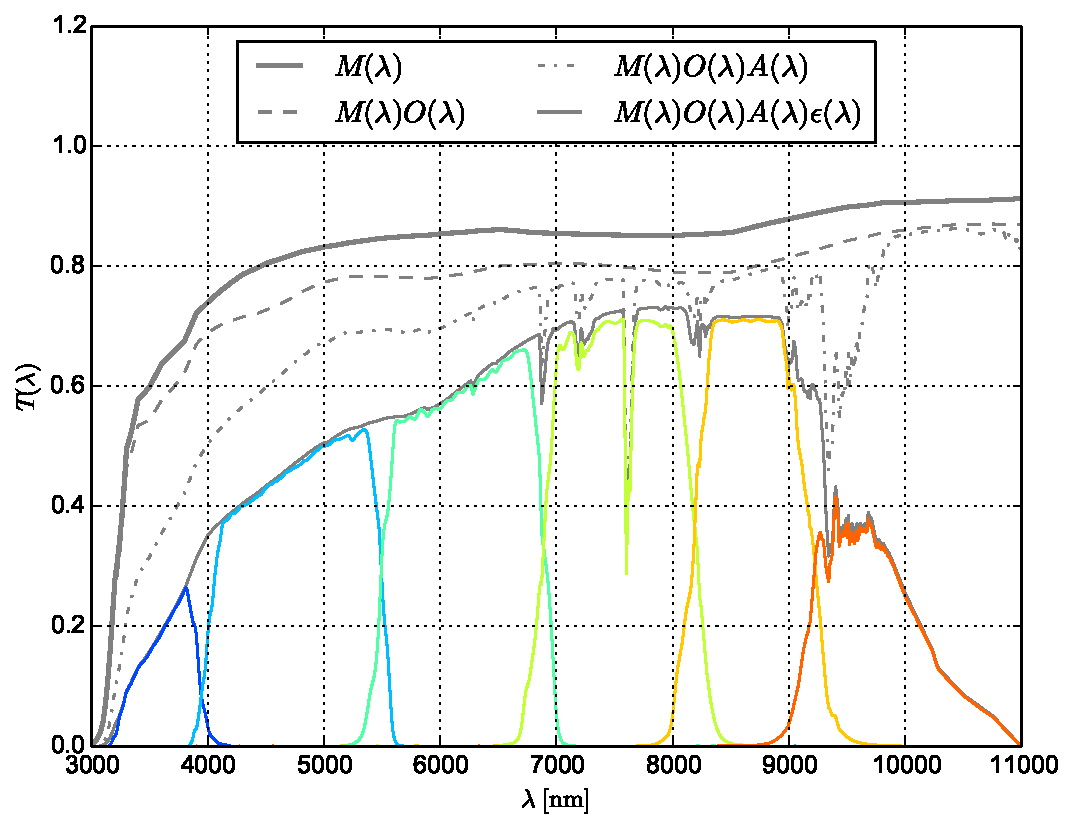
\includegraphics[width=0.45\linewidth]{lse_40_passbands.pdf}}
\subfigure[SMTN-002]{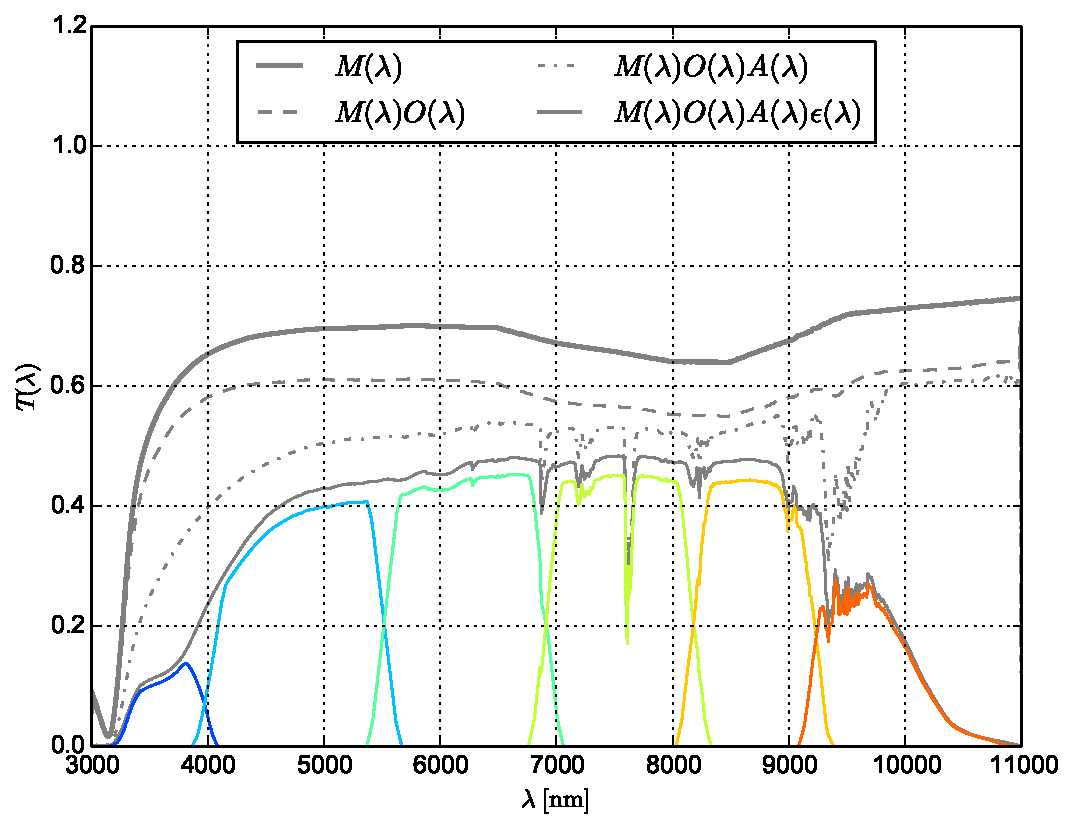
\includegraphics[width=0.45\linewidth]{smtn002_passbands.pdf}}
\caption{Instrument passbands}
\end{center}
\end{figure}


\begin{figure}[t]
\begin{center}
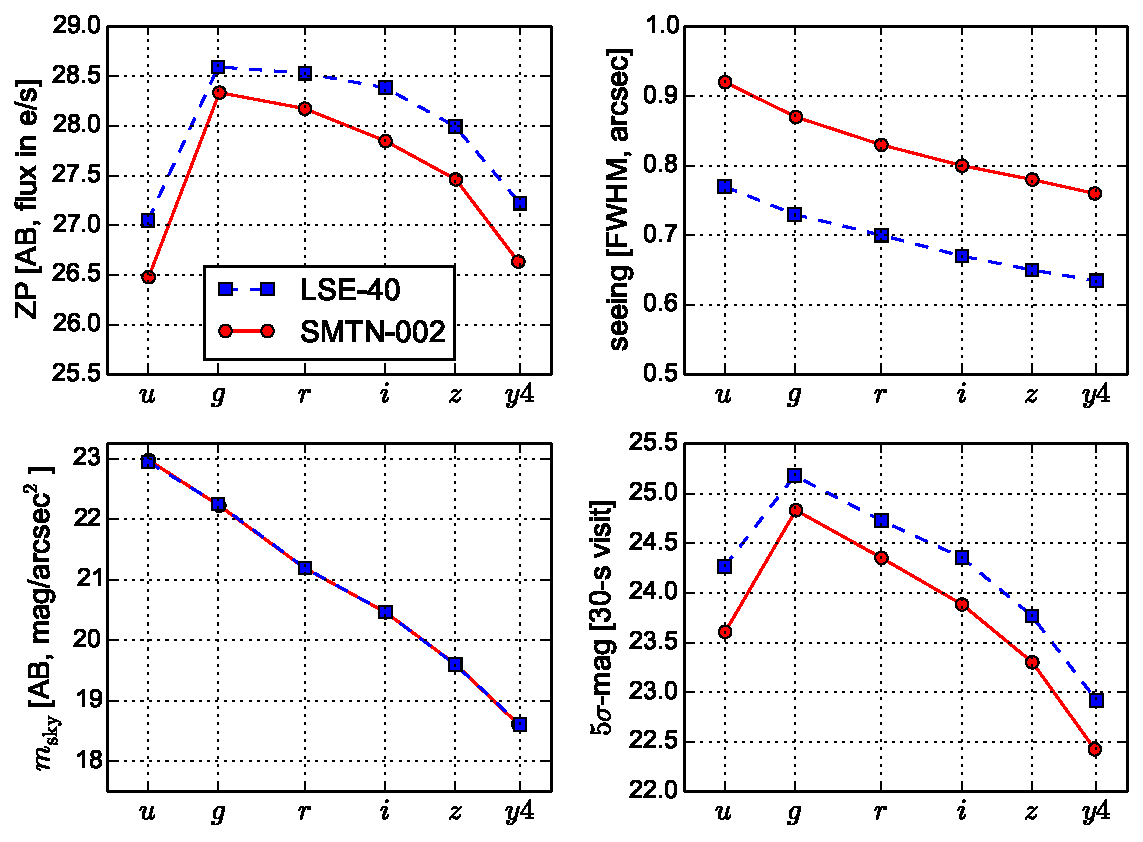
\includegraphics[width=\linewidth]{lsst_model_summary.pdf}
\caption{Zero-points, median seeing, dark sky mags and limiting mags}
\end{center}
\end{figure}



\end{document}
% ======================================================================
% 
